\section{Implementaci\'on del cl\'uster Spark con HDFS}

\subsection{Arquitectura desplegada}

La arquitectura multimodo implementada se compone de tres maquinas virtuales Ubuntu:

\begin{itemize}
    \item \textbf{master}: ejecuta NameNode de HDFS, ResourceManager de YARN y participa como nodo de computo.
    \item \textbf{slave1}: ejecuta DataNode y NodeManager.
    \item \textbf{slave-base}: ejecuta DataNode y NodeManager.
\end{itemize}

El almacenamiento distribuido se gestiono con HDFS y la ejecucion de Spark se realizo sobre YARN. La entrada principal del proyecto se ubico en \texttt{hdfs:///mdjm/input/dataset\_vf\_3.csv} y la salida completa de verificacion en \texttt{hdfs:///mdjm/output\_3nodes\_verify\_20260707\_2325}.

\subsection{Versiones y recursos}

\begin{table}[H]
    \centering
    \caption{Versiones y configuracion base del entorno.}
    \label{tab:versions}
    \begin{tabularx}{\textwidth}{lX}
        \toprule
        \textbf{Componente} & \textbf{Configuracion verificada} \\
        \midrule
        Hadoop & 3.3.0 \\
        Spark & 3.4.0, Scala 2.12.17 \\
        Gestor de recursos & YARN, Capacity Scheduler \\
        Nodos activos & 3: \texttt{master}, \texttt{slave1}, \texttt{slave-base} \\
        Recursos YARN totales & 8 GB de memoria y 4 vcores \\
        Recursos master & 4 GB, 2 vcores \\
        Recursos por worker & 2 GB, 1 vcore por nodo \\
        Interfaz YARN & \url{http://192.168.1.48:8088} \\
        Interfaz NameNode & \url{http://192.168.1.48:9870} \\
        Spark UI en ejecucion & \url{http://192.168.1.48:4040} \\
        \bottomrule
    \end{tabularx}
\end{table}

\subsection{Pasos principales de implementacion}

Los pasos aplicados fueron:

\begin{enumerate}
    \item Verificar conectividad entre los tres nodos mediante nombres de host \texttt{master}, \texttt{slave1} y \texttt{slave-base}.
    \item Revisar espacio disponible y crear directorios temporales para Spark en cada nodo.
    \item Configurar HDFS con NameNode en el master y DataNodes en los workers.
    \item Configurar YARN con ResourceManager en el master y NodeManagers en los tres nodos.
    \item Instalar y validar Spark en \texttt{/opt/spark}.
    \item Definir variables de entorno: \texttt{SPARK\_HOME}, \texttt{HADOOP\_CONF\_DIR}, \texttt{YARN\_CONF\_DIR} y \texttt{SPARK\_LOCAL\_DIRS}.
    \item Subir el dataset a HDFS y ejecutar el jar \texttt{arbitrios-mdjm.jar} con \texttt{spark-submit --master yarn}.
    \item Monitorear la ejecucion con YARN UI, Spark UI, comandos \texttt{yarn node -list -showDetails} y \texttt{htop}.
\end{enumerate}

\subsection{Pruebas de configuracion y conectividad}

La conectividad entre Hadoop, YARN y Spark se valido desde el nodo maestro. La prueba principal fue consultar YARN con \texttt{yarn node -list -showDetails}, ya que este comando confirma que los tres NodeManagers se comunican con el ResourceManager y reportan estado \texttt{RUNNING}. Esto demuestra que el master reconoce a \texttt{slave1} y \texttt{slave-base} como nodos disponibles para ejecutar contenedores.

Adicionalmente, se revisaron los archivos de configuracion de Hadoop y Spark:

\begin{itemize}
    \item \texttt{workers}: lista los nodos que participan como workers.
    \item \texttt{core-site.xml}: define \texttt{fs.defaultFS} apuntando al NameNode del master.
    \item \texttt{hdfs-site.xml}: configura almacenamiento distribuido y replicacion.
    \item \texttt{yarn-site.xml}: define ResourceManager, NodeManagers, memoria y vcores.
    \item \texttt{spark-env.sh} y \texttt{spark-defaults.conf}: conectan Spark con Hadoop/YARN mediante \texttt{HADOOP\_CONF\_DIR}, \texttt{YARN\_CONF\_DIR} y \texttt{spark.master yarn}.
\end{itemize}

Estas pruebas son importantes porque no basta con instalar Spark en cada maquina; Spark debe leer la configuracion de Hadoop para ubicar HDFS y debe enviar sus aplicaciones a YARN para que los ejecutores se distribuyan entre los nodos.

\subsection{Evidencias visuales de ejecucion}

\begin{figure}[H]
    \centering
    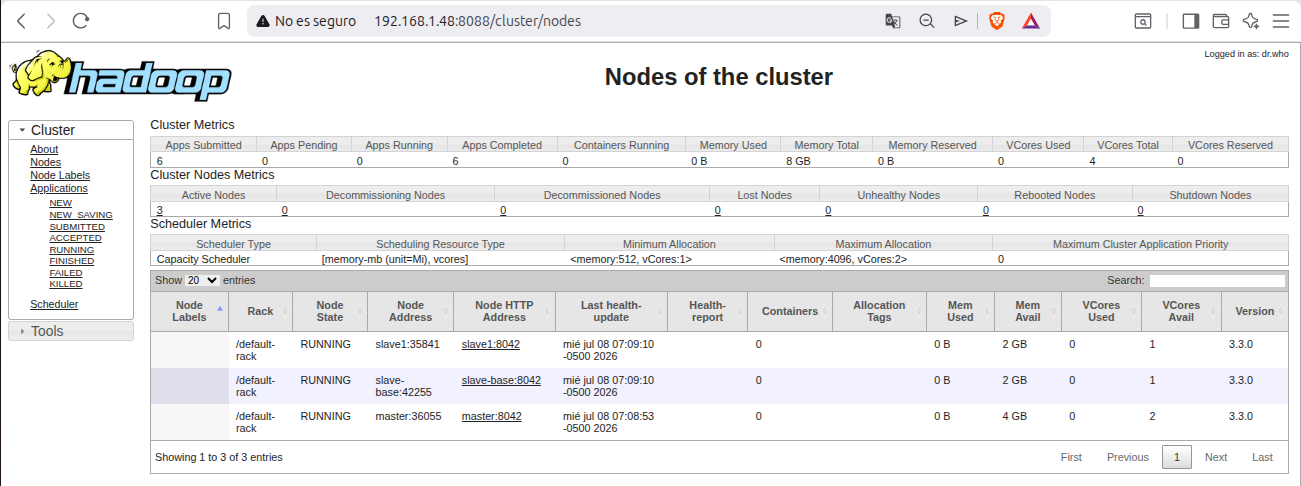
\includegraphics[width=\textwidth]{ImgMultiNodo/Nodes_02_yarn_nodos_cluster_activos.png}
    \caption{Interfaz YARN con los tres nodos activos: \texttt{master}, \texttt{slave1} y \texttt{slave-base}.}
    \label{fig:yarn-nodes}
\end{figure}

\begin{figure}[H]
    \centering
    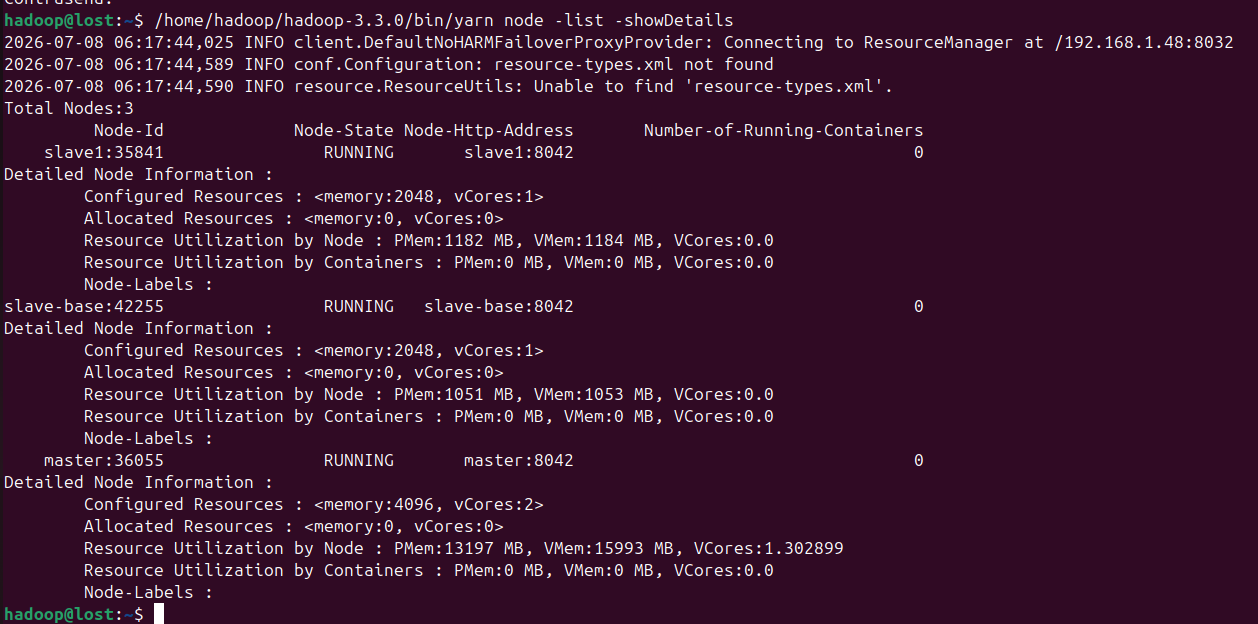
\includegraphics[width=\textwidth]{ImgMultiNodo/VerificarCluster_Los3Activos.png}
    \caption{Verificacion por terminal de los tres nodos activos mediante \texttt{yarn node -list -showDetails}.}
    \label{fig:yarn-terminal-nodes}
\end{figure}

\begin{figure}[H]
    \centering
    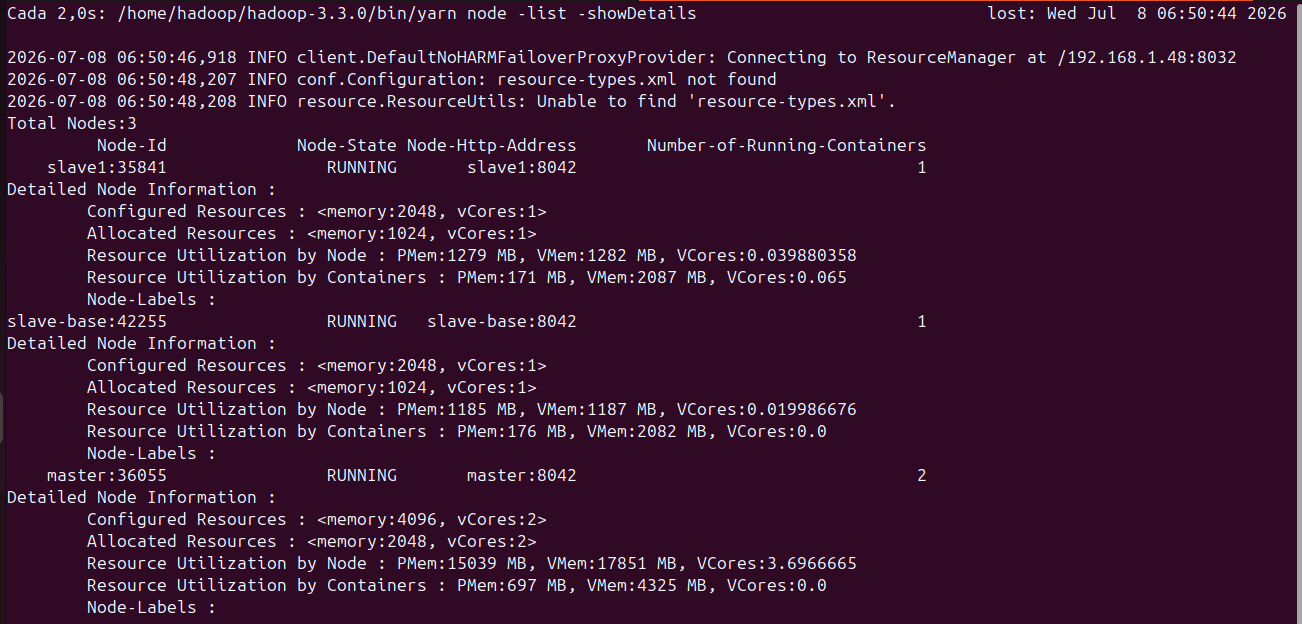
\includegraphics[width=\textwidth]{ImgMultiNodo/yarn_node_showdetails_live.png}
    \caption{Monitoreo por terminal durante la ejecucion distribuida: contenedores activos y recursos asignados por nodo.}
    \label{fig:yarn-live}
\end{figure}

\begin{figure}[H]
    \centering
    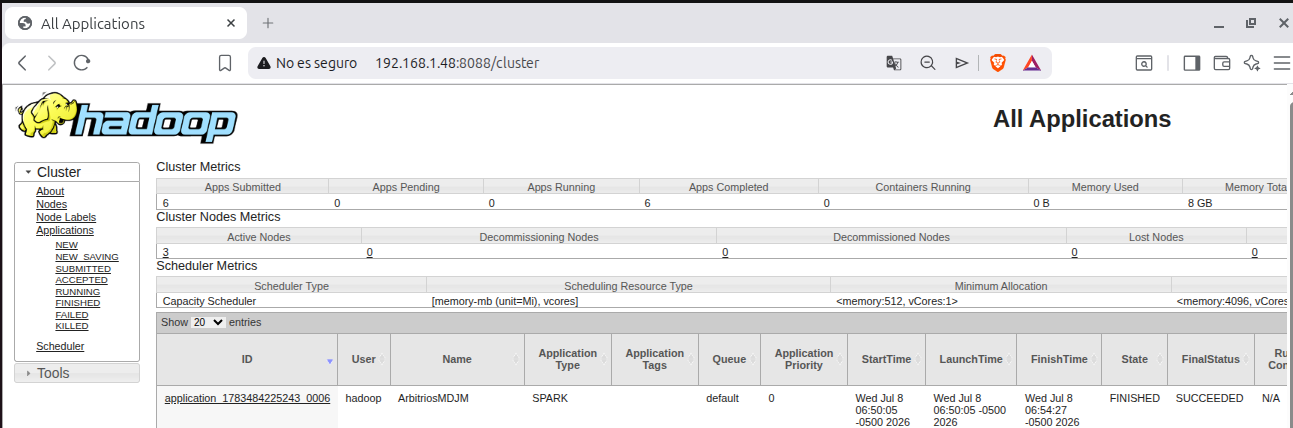
\includegraphics[width=\textwidth]{ImgMultiNodo/cluster_01_yarn_aplicacion_spark_succeeded.png}
    \caption{Aplicacion Spark \texttt{ArbitriosMDJM} finalizada exitosamente en YARN.}
    \label{fig:yarn-succeeded}
\end{figure}

\begin{figure}[H]
    \centering
    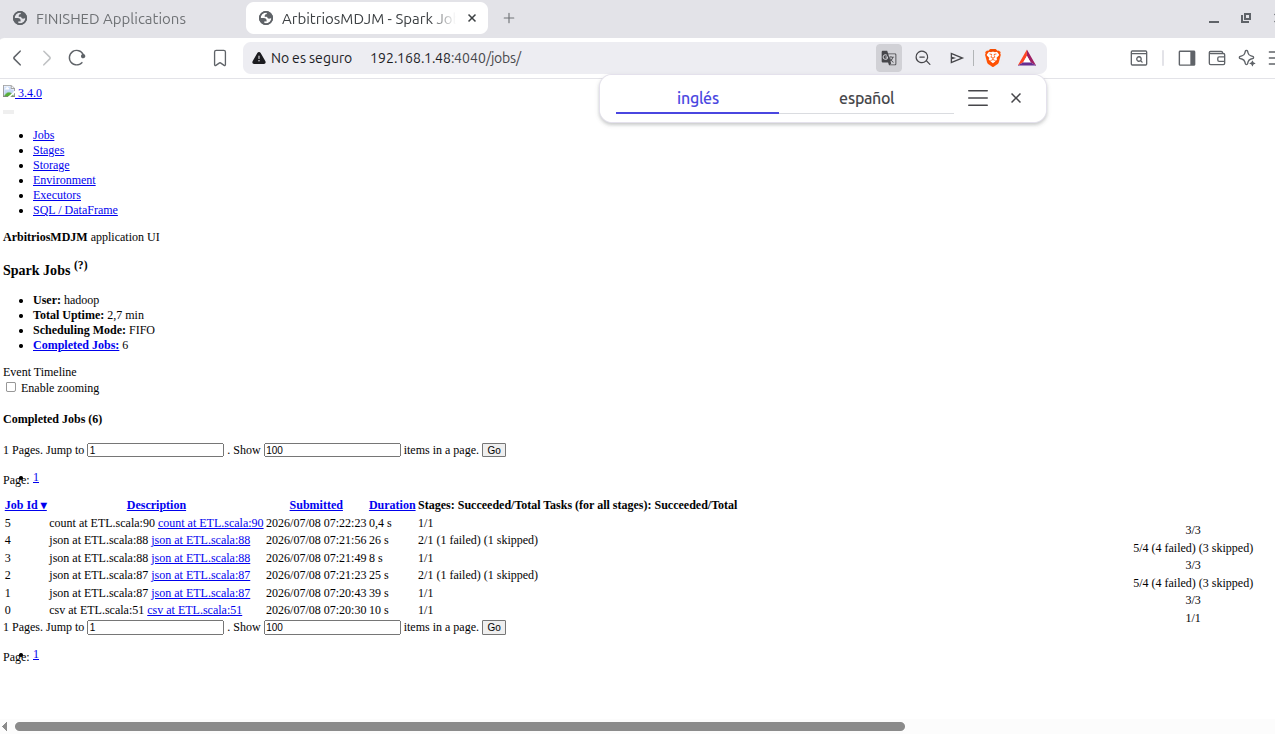
\includegraphics[width=\textwidth]{ImgMultiNodo/SparkUIETL.png}
    \caption{Spark UI durante la etapa ETL, con trabajos completados para lectura, transformacion y escritura en JSON.}
    \label{fig:spark-ui-etl}
\end{figure}
